\section{Task Formulation}
\label{sec:task_formulation}

\paragraph{Setting.} We consider \textbf{document-level} visual retrieval. The input is a text query $q$ and a corpus $\mathcal{D} = \{d_1, d_2, \ldots, d_M\}$ of $M$ documents. Each document $d_i$ is a multi-page visual object: $d_i = \{p_1^{(i)}, p_2^{(i)}, \ldots, p_{N_i}^{(i)}\}$, where $p_j^{(i)}$ denotes the $j$-th page of document $i$ (e.g., a page image). The system assigns a relevance score $s(q, d_i) \in \mathbf{R}$ to each document and returns a ranking over $\mathcal{D}$. The goal is to rank relevant documents above irrelevant ones, where relevance is defined at the \emph{document} level.

\paragraph{Differences from page-level retrieval.} Two issues distinguish document-level from page-level retrieval. (1) \textbf{Representation compression:} A document has a variable number of pages $N_i$. Efficient retrieval therefore requires a representation whose size does not grow linearly with $N_i$. Page-level methods index each page separately and incur $\mathcal{O}(\sum_i N_i \cdot T)$ storage (with $T$ vectors per page), which is prohibitive at scale. (2) \textbf{Multi-positive document supervision:} At the document level, many queries naturally have multiple relevant documents (e.g., several reports on the same policy). Training with a single positive per query mislabels other relevant documents as negatives and degrades learning. We therefore need objectives that support multiple positives per query.

\paragraph{Page-aggregation baseline.} A straightforward baseline aggregates page scores into a document score: $s(q, d_i) = \mathrm{Agg}_{p \in d_i}\, s(q, p)$ (MaxP). This does not reduce index size. When relevance is \emph{distributed} across pages, no single page has a dominant score, so MaxP tends to underrank such documents. DocPC instead builds one composite representation per document and scores it directly.

\paragraph{Relevance distribution analysis.} We analyze page-wise relevance ranks produced by zero-shot ColQwen on a randomly sampled 10\% subset of the DocViRe training split (Figure~\ref{fig:relevance-distribution}). The first two pages achieve the best average ranks, indicating that early pages often carry stronger document-level signals. This motivates early-page-aware selection strategies in DocPC.

\begin{figure}[t]
  \centering
  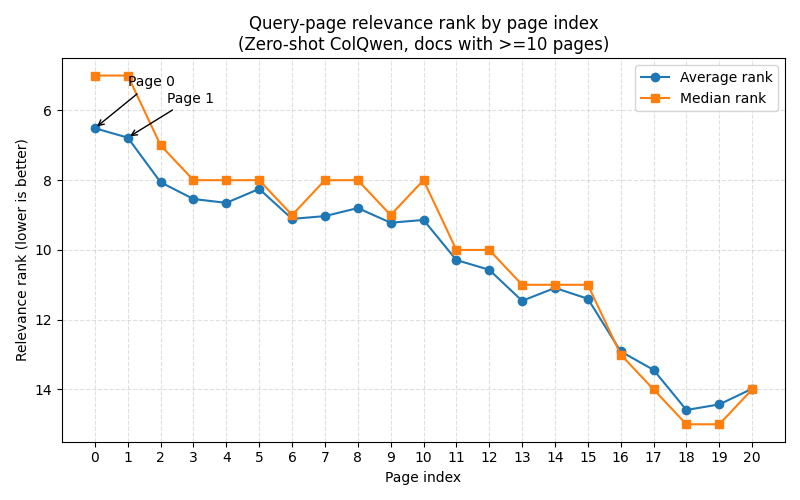
\includegraphics[width=\columnwidth]{figures/相关性排名.png}
  \caption{Average relevance rank by page index on a randomly sampled 10\% subset of the DocViRe training split. For relevant query-document pairs, we compute the page-wise relevance rank produced by zero-shot ColQwen and report the first 20 page positions. Lower rank indicates stronger relevance. The first two pages are ranked most favorably, suggesting that early pages contain strong document-level signals.}
  \label{fig:relevance-distribution}
\end{figure}